%========================================================================================
% TU Dortmund, Informatik Lehrstuhl VII
%========================================================================================

\chapter{Klassendiagramm}
\label{anhangA}
%
Abbildung \ref{fig:classDiagram} enthält alle in der Anwendung vorkommenden Klassen. Der Übersichtlichkeit halber, wurden die Funktionen und Member der einzelnen Klasse ausgelassen. 

\begin{figure}[h]
\centering
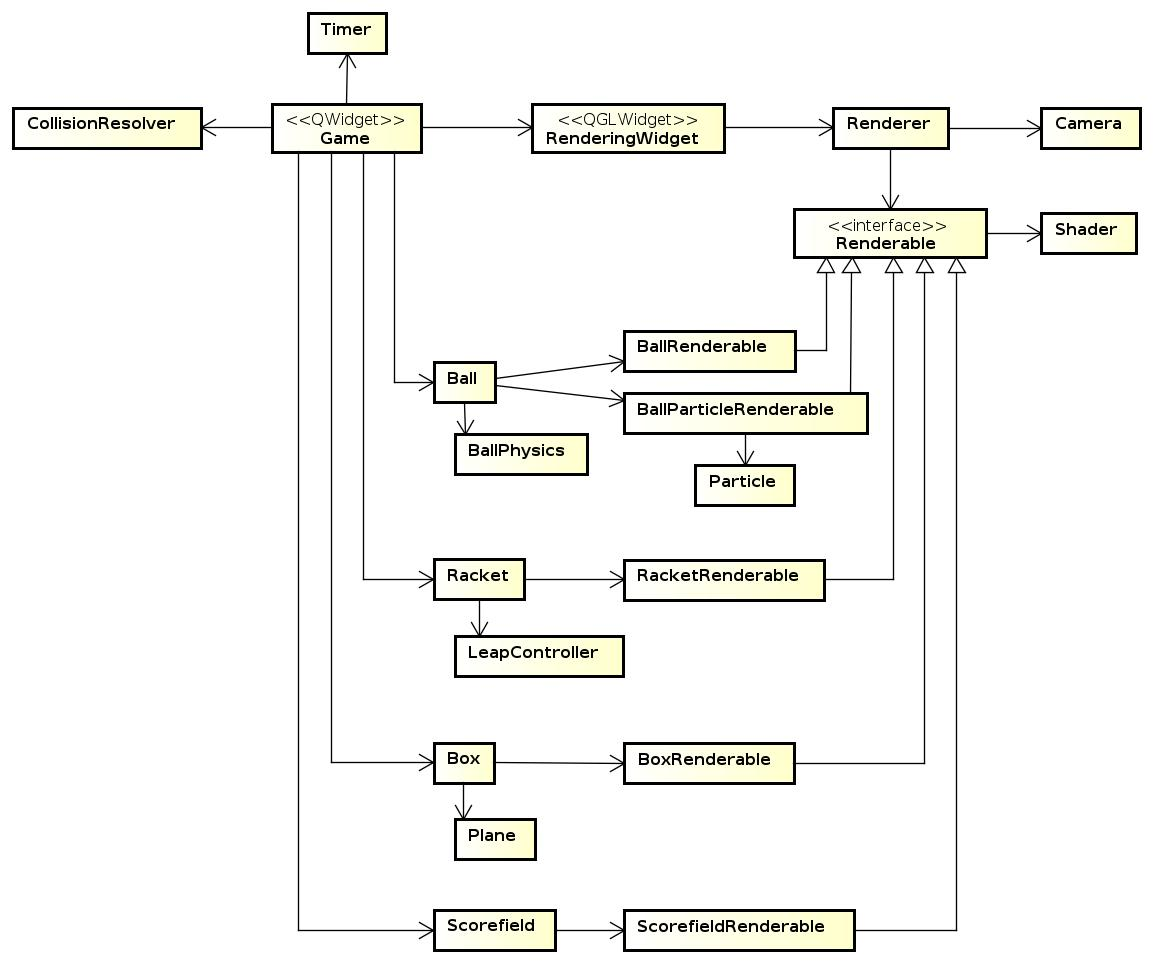
\includegraphics[width=0.9\linewidth]{bilder/classDiagram}
\caption{Klassendiagramm}
\label{fig:classDiagram}
\end{figure}

